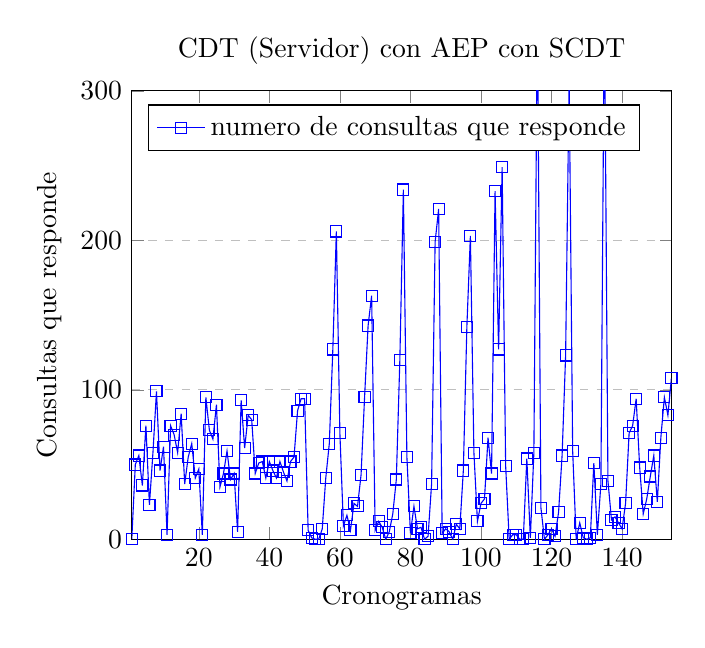
\begin{tikzpicture}
\begin{axis}[
    title={CDT (Servidor) con AEP con SCDT},
    xlabel={Cronogramas},
    ylabel={Consultas que responde},
    xmin=1, xmax=154,
    ymin=0, ymax=300,
    xtick={},
    ytick={},
    legend pos=north west,
    ymajorgrids=true,
    grid style=dashed,
]

\addplot[
    color=blue,
    mark=square,
    ]
    coordinates {
   %CARGA DE TRABAJO Servidor
(1,0)
(2,50)
(3,56)
(4,36)
(5,76)
(6,23)
(7,58)
(8,99)
(9,46)
(10,62)
(11,3)
(12,76)
(13,70)
(14,58)
(15,84)
(16,37)
(17,55)
(18,64)
(19,41)
(20,47)
(21,3)
(22,95)
(23,73)
(24,67)
(25,90)
(26,35)
(27,44)
(28,59)
(29,40)
(30,44)
(31,5)
(32,93)
(33,61)
(34,83)
(35,80)
(36,44)
(37,51)
(38,52)
(39,41)
(40,52)
(41,46)
(42,41)
(43,52)
(44,45)
(45,39)
(46,52)
(47,55)
(48,86)
(49,94)
(50,94)
(51,6)
(52,1)
(53,0)
(54,0)
(55,7)
(56,41)
(57,64)
(58,127)
(59,206)
(60,71)
(61,9)
(62,16)
(63,6)
(64,24)
(65,22)
(66,43)
(67,95)
(68,143)
(69,163)
(70,6)
(71,12)
(72,8)
(73,0)
(74,5)
(75,17)
(76,40)
(77,120)
(78,234)
(79,55)
(80,4)
(81,22)
(82,7)
(83,8)
(84,0)
(85,2)
(86,37)
(87,199)
(88,221)
(89,4)
(90,7)
(91,5)
(92,0)
(93,10)
(94,7)
(95,46)
(96,142)
(97,203)
(98,58)
(99,12)
(100,24)
(101,27)
(102,68)
(103,44)
(104,233)
(105,127)
(106,249)
(107,49)
(108,0)
(109,3)
(110,3)
(111,0)
(112,0)
(113,54)
(114,1)
(115,58)
(116,355)
(117,21)
(118,0)
(119,3)
(120,7)
(121,2)
(122,18)
(123,56)
(124,123)
(125,309)
(126,59)
(127,0)
(128,11)
(129,1)
(130,0)
(131,1)
(132,51)
(133,3)
(134,37)
(135,361)
(136,39)
(137,13)
(138,15)
(139,11)
(140,7)
(141,24)
(142,71)
(143,76)
(144,94)
(145,48)
(146,17)
(147,27)
(148,42)
(149,56)
(150,25)
(151,68)
(152,95)
(153,83)
(154,108)
(155,66)
(156,306)
    };
    \legend{numero de consultas que responde}

\end{axis}
\end{tikzpicture}
